\documentclass[tikz]{standalone}
%\usepackage[usenames]{color} %used for font color
%\usepackage{amssymb} %maths
%\usepackage{amsmath} %maths
%\usepackage[utf8]{inputenc} %useful to type directly diacritic characters
%\usepackage{tikz}
%\usepackage{lscape}
\usetikzlibrary{shapes,arrows,snakes,backgrounds,chains}

\tikzstyle{AG} = [rectangle, draw, fill=black!21, 
    text width=6em, text centered, minimum height=4em]
\tikzstyle{AGwide} = [rectangle, draw, fill=black!21, 
    text width=8em, text centered, minimum height=4em]
\tikzstyle{PO} = [rectangle, draw, fill=black!10, 
    text width=6em, text centered, rounded corners, minimum height=4em]
\tikzstyle{POwide} = [rectangle, draw, fill=black!10, 
    text width=8em, text centered, rounded corners, minimum height=4em]
\tikzstyle{line} = [draw, -latex']
\tikzstyle{cloud} = [draw, ellipse,fill=black!1, node distance=3cm, text width=3.5em, text centered,
    minimum height=2em]
\begin{document}
\pagestyle{empty}
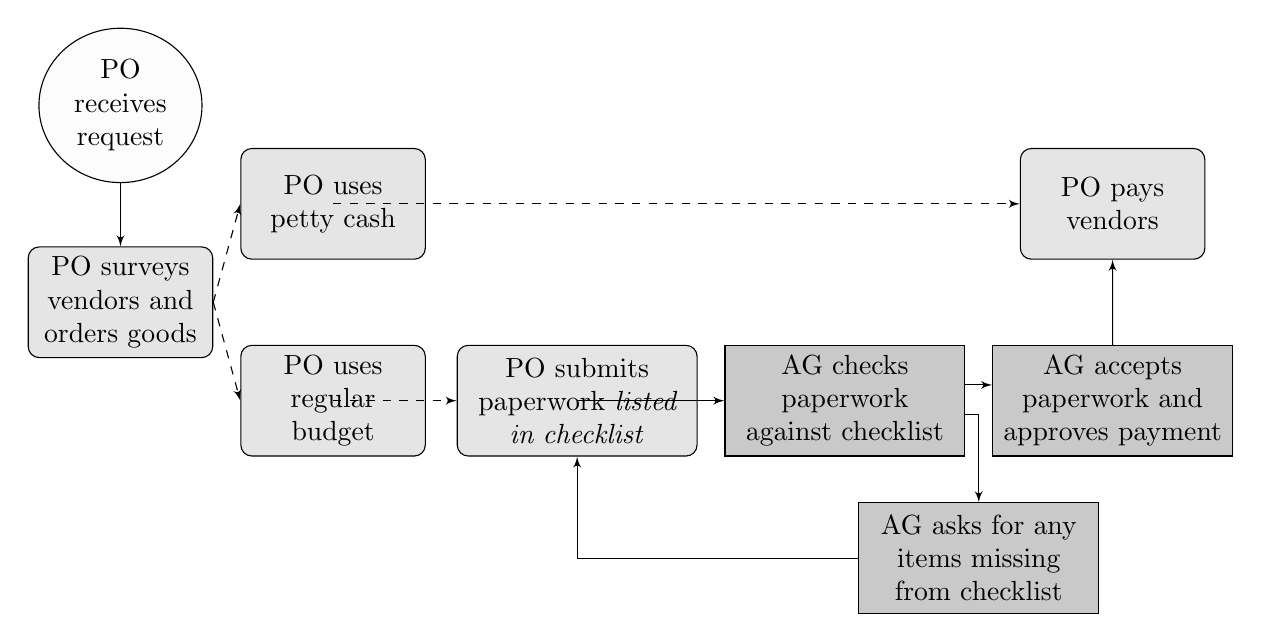
\begin{tikzpicture}[node distance = 2cm, auto]
 \node [PO] (survey) {PO surveys vendors and orders goods};
 \node at (2.7,1.25) [PO, name=pettycash] {PO uses petty cash};
  \node at (2.7,-1.25) [PO, name=regbudg] {PO uses regular budget};
    \node [cloud, above of=survey, node distance=2.5cm] (request) {PO receives request};
    \node [PO, right of=pettycash, node distance = 9.9cm] (pay) {PO pays vendors};
    \node [POwide, right of=regbudg, node distance=3.1cm] (paperwork) {PO submits paperwork \emph{listed in checklist}};
    \node [AGwide, right of=paperwork, node distance=3.4cm] (examine) {AG checks paperwork against checklist};
    \node at (10.9, -3.25) [AGwide, name=reject] {AG asks for any items missing from checklist};
    \node [AGwide, right of=examine, node distance=3.4cm, name=appr] (appr) {AG accepts paperwork and approves payment};
 \path [line,dashed] (survey.east) -- (pettycash.west);
	\path [line,dashed] (pettycash) |- (pay);
    \path [line,dashed] (survey.east) -- (regbudg.west);
    \path [line,dashed] (regbudg) |- (paperwork);
    \path [line] (paperwork) |- (examine);
    \path [line] ([yshift=.2cm]examine.east) -- ([yshift=.2cm]appr.west);
    \path [line] ([yshift=-.2cm]examine) -| (reject.north);
    \path [line] (reject) -| (paperwork);
    \path [line] (appr) -- (pay);
    \path [line] (request) -- (survey);
\end{tikzpicture}
\end{document}